\documentclass{article} % For LaTeX2e
\usepackage{nips15submit_e,times}
\usepackage{hyperref}
\usepackage{url}
\usepackage{graphicx}
\usepackage{amsfonts}
\usepackage{amssymb}
\usepackage{float}
\usepackage{listings}
\usepackage{xcolor}
\usepackage{amsmath}
%\documentstyle[nips14submit_09,times,art10]{article} % For LaTeX 2.09


\title{Problem Set 5 for Machine Learning 15 Fall}


\author{
Jingyuan Liu\\
AndrewId: jingyual\\
\texttt{jingyual@andrew.cmu.edu} \\
}


\newcommand{\fix}{\marginpar{FIX}}
\newcommand{\new}{\marginpar{NEW}}
\newcommand{\argmin}{\arg\!\min}
\newcommand{\norm}[1]{\left\lVert #1 \right\rVert}
\newcommand{\abs}[1]{\left\lvert #1 \right\rvert}
\newcommand{\inner}[1]{\left\langle #1 \right\rangle}

\nipsfinalcopy % Uncomment for camera-ready version


\begin{document}
\maketitle



\section{Gaussian Graphical Model}


\subsection{Derive $\phi_{ij} (x_i, x_j)$ and $\phi_i (x_i)$}
%\begin{figure}[!htbp]
%\begin{center}
%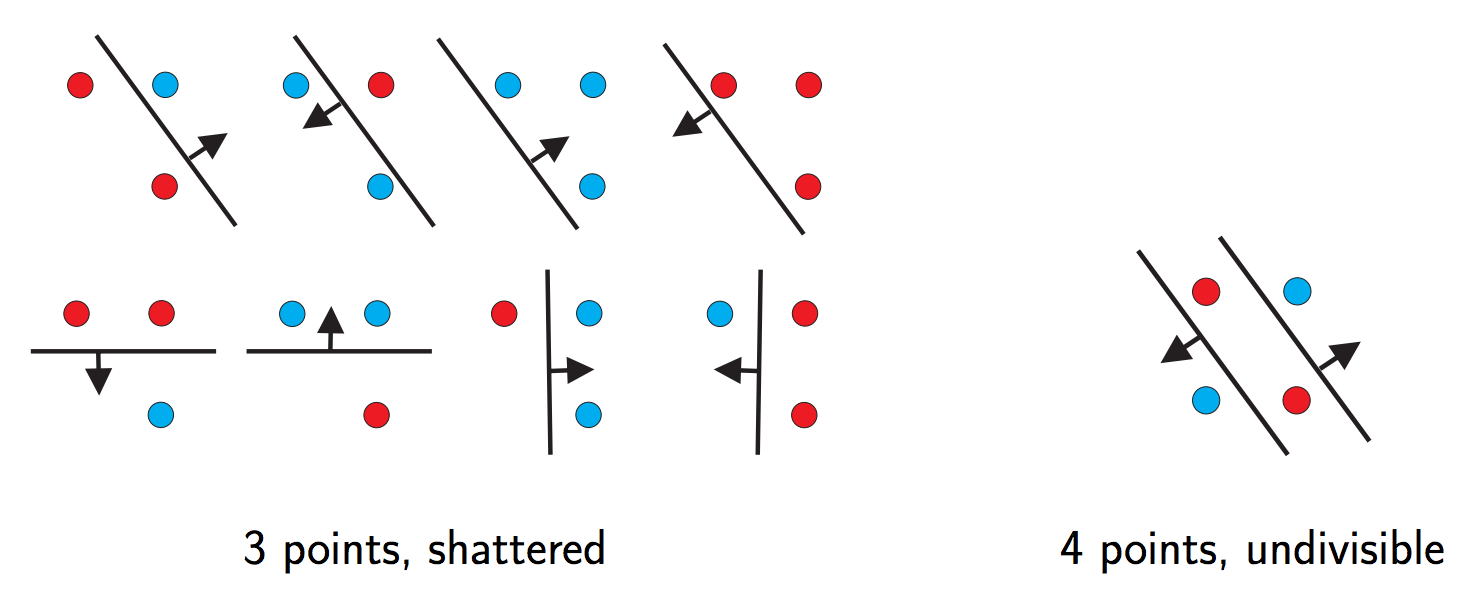
\includegraphics[width=80mm]{pic/q11.png}
%\end{center}
%\caption{The representation of $VCdim(h_2)$}
%\end{figure}

\begin{equation}
P(X \mid \mu, \Sigma) = \frac{1}{\sqrt{(2\pi)^n \Sigma}}
exp (-\frac{1}{2} (x-\mu)^T \Sigma^{-1} (x-\mu))
\end{equation}

\begin{equation}
P(X \mid \mu, \Omega) \propto exp (-\frac{1}{2} X^T \Omega X + (\Omega \mu)^T X)
\end{equation}

\begin{equation}
\qquad \qquad =
\prod_{i \in V} exp (-\frac{1}{2} x_i^T \Omega_{ii} x_i + (\Omega \mu)_i^T x_i)
\prod_{(i, j) \in E} exp( -\frac{1}{2} x_i^T \Omega_{ij} x_j)
\end{equation}

\begin{equation}
\psi_{ij} (x_i, x_j) =
exp( -\frac{1}{2} x_i^T \Omega_{ij} x_j)
, \quad
\psi_{i} (x_i) =
exp (-\frac{1}{2} x_i^T \Omega_{ii} x_i + (\Omega \mu)_i^T x_i)
\end{equation}


\subsection{Prove $(i,j ) \notin E \iff X_i \perp X_j | X_{V\backslash\{i,j\}}$}
If $(i, j) \notin E$, there is no edge between node i
and node j, then we can get:

\begin{equation}
\Omega_{ij} = 0, \qquad \psi_{ij} (x_i, x_j) = 1
\end{equation}

\begin{equation}
P (x_i, x_j \mid V\backslash\{i,j\}, \mu, \Omega) = \psi_{ij}' (x_i, x_j)
= \psi_{ij} (x_i, x_j) \cdot \psi_i (x_i)^{\frac{1}{n(i)}}
\cdot \psi_j (x_j)^{\frac{1}{n(j)}}
\end{equation}

\begin{equation}
\qquad \qquad=
\psi_i (x_i)^{\frac{1}{n(i)}}
\cdot \psi_j (x_j)^{\frac{1}{n(j)}}
\end{equation}

\begin{equation}
\qquad \qquad =
P (x_i\mid V\backslash\{i\}, \mu, \Omega)
\cdot P (x_j\mid V\backslash\{j\}, \mu, \Omega)
\end{equation}

\begin{equation}
\qquad \qquad \qquad =
P (x_i\mid V\backslash\{i,j\}, \mu, \Omega)
\cdot P (x_j\mid V\backslash\{i,j\}, \mu, \Omega)
\end{equation}

We can notice the above process could be inverse, which means if we know that
the two points are independent, we could get that there is no edge between these
two nodes. Therefore, we could prove the conclusion.



\section{Sampling}


\subsection{Inverse Sampling}
\textbf{2.1.1 Prove Inverse Sampling}

First, for y' $\in$ R, we have:

\begin{equation}
P (h^{-1} (z) <= y') = P (inf {y: h(y) = z} < y')
\end{equation}

\begin{equation}
\qquad =
P (z <= h(y')) = h (y')
\end{equation}

Second, for $0 < z'< 1$, we have:

\begin{equation}
P(h(y) < z') = P(y < h^{-1} (z')) = z'
\end{equation}

Therefor, we could prove that inverse sampling is reasonable. The drawback
could be:

(1) In real application, it would require a closed form expression for F(x),
which means we would need do normalization sometimes.

(2) In real application, we need to konw the p(y) to do sampling.

\textbf{2.1.2 Find the Cauchy distribution transfermation}

Given the density function, we could derive:

\begin{equation}
h (y) = \int_{-\infty}^y p(y') dy' = \frac{1}{2} + \frac{1}{\pi} arctan(y)
\end{equation}

\begin{equation}
y = g (z) = h^{-1} (z) = tan(\pi (z - \frac{1}{2}))
\end{equation}


\subsection{Rejection Sampling}












\subsection{Markov Chain Monte Carlo}
From above questions, we could get:

\begin{equation}
\epsilon <= e^{-2 \sum_t \gamma_t^2}
\end{equation}

With the smallest margin of $\gamma$, we could transfer to

\begin{equation}
\epsilon <= e^{-2 T \gamma^2}
\end{equation}

\begin{equation}
T = O (\frac{-log (\epsilon)}{\gamma^2})
\end{equation}


\subsection{implementation}
For each h, we choose the classifier with smallest error in each
iteration. The result is:

\begin{table}[h]
\renewcommand{\arraystretch}{1.5}
\centering
\begin{tabular}{|c|c|c|c|c|c|c|c|c|c|c|c|c|}
\hline 
$ t $ 
& $ \epsilon_t $ 
& $ \alpha_t $ 
& $ D_t(1) $ 
& $ D_t(2) $ 
& $ D_t(3) $
& $ D_t(4) $
& $ D_t(5) $
& $ D_t(6) $
& $ D_t(7) $
& $ D_t(8) $
& $ D_t(9) $ 
& $ err_S(H) $ \\
\hline 
1 &0.222 &0.626 &0.11 &0.11 &0.11 &0.11 &0.11
&0.11 &0.11 &0.11 &0.11 &0.222 \\
\hline 
2 &0.143 &0.896 &0.071 &0.071 &0.071 &0.071 &0.071
&0.071 &0.071 &0.25 &0.25 &0.222 \\
\hline 
3 &0.125 &0.973 &0.042 &0.042 &0.042 &0.042 &0.25
&0.25 &0.042 &0.146 &0.146 &0 \\
\hline 
\end{tabular}
\caption{AdaBoost results}
\label{tbl:boost}
\end{table}

The classfication rule: first, if $x > 2.5$, pos; second, if $x > 3.5$,
pos; third, if $x < 4.5$, pos.



\section{Gaussian Mixture Model}


\subsection{Show the expectation}
\begin{equation}
E (x) = \int p(x) dx = \sum_k p(x_k) x_k
\end{equation}

\begin{equation}
\qquad \qquad \qquad \qquad
= \sum_k \pi_k E_k (x)
\end{equation}

We know that for each k, the implict distribution of x is a Gaussian
distribution, and $E_k (x) = \mu_k$, $\mu_k$ is the mean of the kth guassian
distribution, so we have:

\begin{equation}
\qquad \qquad
E (x) = \sum_k \pi_k \mu_k
\end{equation}


\subsection{Show the covariance}
\begin{equation}
cov (x) = E (x x^T) - E (x) E(x)^T
\end{equation}

\begin{equation}
\qquad \qquad \qquad
= \sum_k \pi_k E_k (x x^T) - E (x) E(x)^T
\end{equation}

\begin{equation}
\qquad \qquad \qquad \qquad
= \sum_k \pi_k (\Sigma_k + \mu_k \mu_k^T) - E (X) E (x)^T
\end{equation}



\section{K-Means}


\subsection{Theory}

\textbf{4.1.1 Prove the lemma}

\begin{equation}
\sum_x \norm{x - s}^2 - \sum_x \norm{x - \bar{x}}^2 =
\sum_x (x^2 -2xs + s^2) - \sum_x (x^2 -2x \bar{x} + \bar{x}^2)
\end{equation}

\begin{equation}
\qquad \qquad \quad
= \sum_x s^2 +2 x \bar{x} - \bar{x}^2 -2\bar{x}s
\end{equation}

Considering that $\bar{x}$ is the center of x points, we have $\sum_x
x\bar{x} = \abs{X} \bar{x}^2$. Therefore:

\begin{equation}
\sum_x s^2 +2 x \bar{x} - \bar{x}^2 -2\bar{x}s
= \sum_x s^2 + \bar{x}^2 - 2 \bar{x} s
= \abs{\mathcal{X}} \norm{\bar{x} - s}^2
\end{equation}

\textbf{4.1.2 Prove the objective}

We could first transfer $w (\mu_k, f; X)$ use $n_k$ to represent all nodes in
kth cluster:

\begin{equation}
w (\mu_k, f; X) = \sum_k \sum_i^n 1(f(x_i) = k) \norm{x_i - \mu_k}^2
\end{equation}

\begin{equation}
= \sum_k \sum_i^{n_k} \norm{x_{ki} - \mu_k}^2
\end{equation}

\begin{equation}
\qquad \quad
= \sum_k \sum_i^{n_k} \frac{1}{n_k} n_k \norm{x_{ki} - \mu_k}^2
\end{equation}

Then we consider the form from $\phi$, for the kth cluster and set the i, we have:
\begin{equation}
\sum_j^{n_k} \norm{x_{ki} - x_{kj}}^2 =
\sum_j^{n_k} x_{ki}^2 - 2x_{ki} x_{kj} + x_{ki}^2
\end{equation}

Using lemma1 and similar tricks in proving lemma1, then we could have:
\begin{equation}
n_k \norm{x_{ki} - \mu_k}^2 = \sum_j \norm{x_{ki} - x_{kj}}^2
\end{equation}

Seperately integrating into the $\phi$ and w, we have:
\begin{equation}
w (\mu_k, f; X) = \sum_k \sum_i^n 1(f(x_i) = k) \norm{x_i - \mu_k}^2
\end{equation}

\begin{equation}
\qquad \qquad \qquad
= \sum_k \sum_i^{n_k} \sum_j^{n_k} \frac{1}{n_k} \norm{x_{ki} - x_{kj}}^2 = \phi
\end{equation}

\textbf{4.1.3 Prove the decrease of objective}

Proving the decrease of objective during each iteration is quite intuive:

\textbf{For step 1}, suppose we have two cluster $\mu_1$ and $\mu_2$. Suppose $\mu_1$ is
closer. Then when we assign the point:

\begin{equation}
\norm{x - \mu_1}^2 < \norm{x - \mu_2}^2
\end{equation}

Therefore, to choose the minimize the total objective w, we should choose
$\mu_1$, which means that step 1 will decrease the objective.

\textbf{For step 2}, we have lemma1:

\begin{equation}
\sum_x \norm{x - s}^2 - \sum_x \norm{x - \bar{x}}^2 =
\abs{X} \norm{\bar{x}-s}^2 > 0
\end{equation}

So we know that, chooseing any other point rather than the ``average'' as center
would cause bigger error, which means that using the ``average'' will decrease
the objective.

\textbf{4.1.4 Prove the convergence with K}

Proving the convergence of $\Omega (K)$ is quite intuitive. When we have the
minimual objective, then in step 1, all the $x_i$ would not change its
assignment of cluster centain. Say we have the $\mu$ and any other $\mu'$, we
would have since that $\Omega$ is the minimual objective.

\begin{equation}
\norm{x - \mu}^2 < \norm{x - \mu'}^2
\end{equation}

For step 2, since all the $x_i$ would not change its assignment, then the $\mu_k =
\frac{1}{n_k} \sum_i x_{ki}$ would not change. So the center would remain the
same.

Therefore, in step 1 and step 2, there would be no change in the assignment and
center, the $\Omega$ would not change with the increase of K

\textbf{4.1.5 Prove the convergence is finite}

The K-means would converge in finite numbers. We know that the center is the
average of all x in a cluster. When we set the K, then the combination of K is a
finite number. In the step 1, the assignment step, the choice of K is
finite. Then in step 2, the change of center is set.

As mentioned from Wikipedia, the time is $O(n^{dk+1} logn)$, with k as the
cluster, d as the dimension of data x and n as the data points number.


\subsection{Implementation}

\textbf{4.2.1 and 4.2.2 Implement the K-means algorithms}

The result is here:

\begin{figure}[!htbp]
\begin{center}
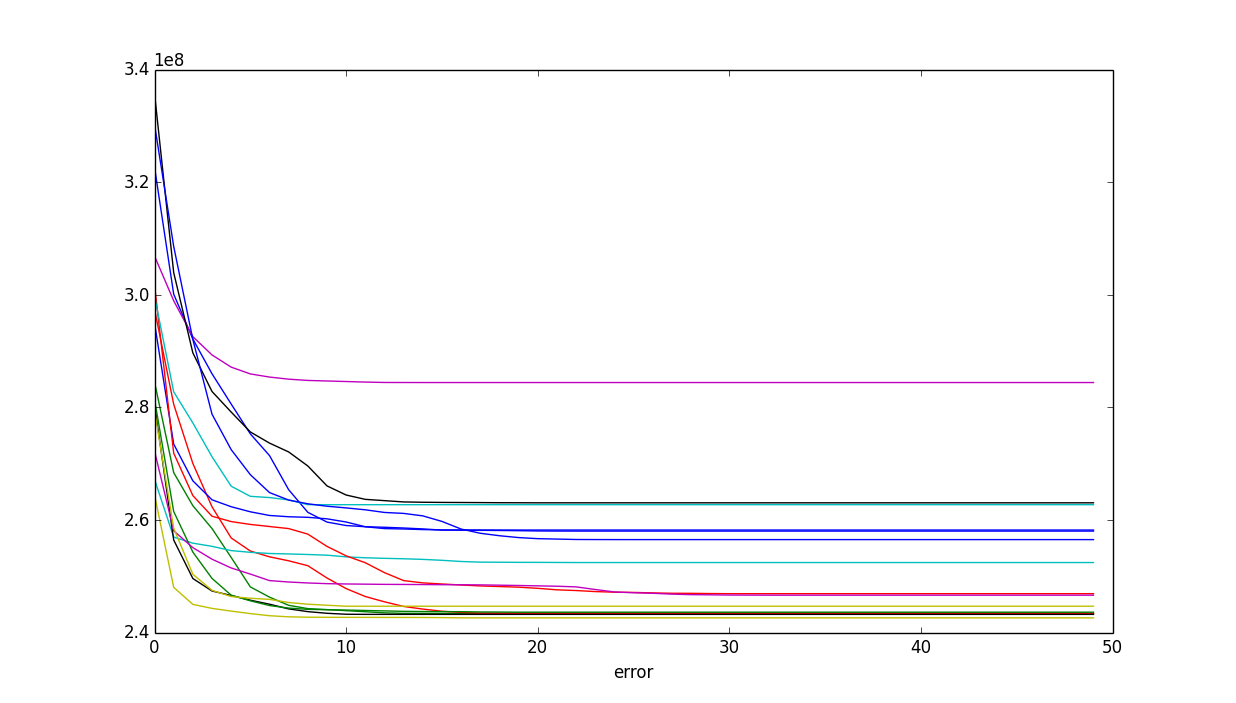
\includegraphics[width=100mm]{pic/q42.png}
\end{center}
\caption{The error over iteration of K-means}
\end{figure}

As we could see from the figure, all the 15 iterations converge within 50
iteration. For most instances, the alogrithm would converge within 15 $\sim$ 20
iterations.



\section{Collaboration}
I did not collaborate with classmates in this assignment. However, I refered to
some code online to finish my K-means algorithms. The link is:
https://github.com/stuntgoat/kmeans.git

Basically, I used the general code structure, the update and assign function.
I implemented my own data read and error plot function. Besides, I change the
interface of the general kmeans function for stop conditions. I also implement
the error function to get the error in each iteration for each cluster.





\end{document}
